\documentclass[12pt]{article}

% Packages for Advanced Formatting
\usepackage{geometry}
\geometry{margin=1in}
\usepackage{amsmath}
\usepackage{amssymb}
\usepackage{tikz}
\usetikzlibrary{calc}
\usepackage{xcolor}
\usepackage{graphicx}
\graphicspath{{images/}}
\usepackage{booktabs}
\usepackage{tabularx}
\usepackage{array}
\usepackage{listings}
\usepackage{setspace}
\usepackage{titlesec}
\usepackage{ragged2e}
\usepackage{indentfirst}
\usepackage{csquotes}
\usepackage{caption}
\usepackage{float}
\usepackage[hidelinks]{hyperref}
\usepackage[style=apa, backend=biber, natbib=true]{biblatex}
\addbibresource{references.bib}

% Color Definitions
\definecolor{dlsugreen}{HTML}{00703C}
\definecolor{codeblue}{RGB}{0,70,140}
\definecolor{codegray}{RGB}{100,100,100}

% Python Code Listings Configuration
\lstset{
  language=Python,
  basicstyle=\small\ttfamily,
  breaklines=true,
  keepspaces=true,
  columns=flexible,
  showstringspaces=false,
  keywordstyle=\color{codeblue},
  commentstyle=\color{dlsugreen},
  stringstyle=\color{purple},
  backgroundcolor=\color{gray!5},
  frame=single,
  framerule=0pt,
  xleftmargin=10pt,
  xrightmargin=10pt,
  aboveskip=15pt,
  belowskip=15pt
}

% APA 7th Edition: Headings & Indents
\titleformat{\section}{\normalfont\Large\bfseries\centering}{\thesection}{1em}{}
\titleformat{\subsection}{\normalfont\large\bfseries}{\thesubsection}{1em}{}
\titlespacing*{\section}{0pt}{12pt}{6pt}
\titlespacing*{\subsection}{0pt}{12pt}{6pt}
\setlength{\bibhang}{0.5in}

% Figure/Table Captions
\captionsetup{
  labelfont=bf,
  labelsep=newline,
  textfont=it,
  justification=raggedright,
  singlelinecheck=false,
  skip=6pt
}

% Math Shortcuts
\newcommand{\usdphp}{USDPHP}
\newcommand{\dxy}{DXY}

% DOCUMENT
\begin{document}
\doublespacing
\RaggedRight
\setlength{\parindent}{0.5in}

\begin{titlepage}
    \centering

    % Top Logo and Name (Inline)
    \vspace*{0.5cm}
    \begin{tabular}{c@{\quad}l}
        \raisebox{-2.0ex}{\includegraphics[height=3.5em]{dlsu_logo.png}} &
        \Large \textbf{\color{dlsugreen} De La Salle University}
    \end{tabular}

    \vfill

    % Central Seal
    \includegraphics[width=0.25\textwidth]{dlsu_logo.png} \\

    \vfill

    % Paper Title
    {\large \textbf{Borrowed Stability: Decomposing Philippine Peso Depreciation\
    Using DXY Normalization and ARIMA Counterfactual Analysis,\
    January 2025 to March 2026}} \\
    \vspace{1.5cm}

    \begin{minipage}{0.8\textwidth}
        \centering
        {\normalsize Department of Financial Management \\ {} De La Salle University, Manila, Philippines}
    \end{minipage}

    \vfill

    {\normalsize By:} \\
    \vspace{0.5cm}
    {\normalsize Aaron Joshua E. Sison \\ {} Undergraduate Student}

    \vfill

    {\normalsize March 28, 2026}
\end{titlepage}

% AUTHOR NOTE
\newpage
\begin{center}
  {\normalsize \textbf{Author Note}}
\end{center}

\hspace{0.5in}{\normalsize
This paper was prepared as part of a quantitative finance research exercise.
Correspondence concerning this paper should be addressed to the author.
No conflicts of interest are declared.
Data and code are available from the author upon request.
Exchange rate data were sourced from Yahoo Finance \citep{yahoophp2026, yahoodxy2026}.
Analysis was performed in Python 3.12 using statsmodels \citep{seabold2010}
and matplotlib \citep{hunter2007}.
}

% ABSTRACT
\newpage
\begin{center}
  \textbf{Abstract}
\end{center}

The Philippine peso presents a misleading image of stability. Since Donald Trump's
inauguration on January 20, 2025, the USD/PHP spot rate rose from 58.15 to 60.21,
a nominal depreciation of 3.54\%. During the same period, the US Dollar Index
(DXY) declined from 108.06 to 100.15, a deterioration of 7.32\% in trade-weighted
dollar strength. This paper decomposes the observed exchange rate movement into
two components: peso-specific depreciation and USD-specific weakness. Two
counterfactual methods are applied. The first is a DXY-normalization procedure
that adjusts the actual USDPHP rate by the ratio of the DXY at inauguration to its
current level, producing a stable-dollar counterfactual rate. The second is an
ARIMA(1,1,1) model with drift, fitted on pre-inauguration data from July 2020 to
January 2025, and projected forward through March 2026. The DXY-normalized rate
for March 27, 2026 is 64.93 PHP/USD, implying a fundamental PHP depreciation of
11.66\% against a stable dollar. The ARIMA forecast yields 60.78 PHP/USD, broadly
consistent with the nominal rate and the pre-existing depreciation trend. The
difference between the normalized counterfactual and the actual rate constitutes a
PHP cushion of 4.72 PHP/USD, representing the portion of peso strength attributable
to dollar weakness rather than peso fundamentals. A hypothesized stable-dollar rate
of approximately 70 PHP/USD is directionally correct but overstated by approximately
5 PHP/USD, equivalent to a DXY decline of 13\% rather than the observed 7.32\%.
The results indicate that the peso is functionally weaker than exchange boards report,
and that BSP reserve operations and OFW remittance flows provide additional suppression
not captured by either model.

\vspace{12pt}
\noindent\textit{Keywords:} Philippine peso, exchange rate decomposition, DXY
normalization, ARIMA, counterfactual analysis, USD weakness, BSP

% BODY
\newpage

\begin{center}
  \textbf{\large Introduction}
\end{center}

\vspace{12pt}

The Philippine peso occupies an uncomfortable position in Southeast Asian currency
markets. Its exchange rate reflects three compounding forces at once: domestic monetary
policy, global dollar dynamics, and the structural peculiarity of an economy whose
external accounts depend heavily on remittance inflows from approximately 10.6 million
overseas Filipino workers (Bangko Sentral ng Pilipinas [\citeauthor{bsp2024}], \citeyear{bsp2024}).
The resulting rate is a composite signal. Separating its components requires an explicit
analytical framework.

This paper addresses one specific decomposition question. Since January 20, 2025,
the US dollar has weakened materially against a trade-weighted basket of major
currencies. The DXY, maintained by ICE Benchmark Administration \citep{ice2023},
declined 7.32\% over this period. The USDPHP rate rose by only 3.54\%. The arithmetic
is consequential: a peso that appears to depreciate modestly against a falling dollar
is, in fundamental terms, depreciating more substantially than the quoted rate implies.
The dollar's weakness is providing cover. This paper quantifies the magnitude of
that cover.

Two analytical instruments are deployed. The first is a DXY-normalization
formula that recalculates the USDPHP rate under a counterfactual of stable dollar
strength. The second is an ARIMA(1,1,1) model fitted on pre-Trump data, projecting
forward what PHP depreciation would look like absent the structural break of the
new administration's trade and fiscal policies. The combination of these approaches
permits a triangulated estimate of the peso's fundamental position.

\section{Objectives}

Five objectives guide this analysis. First, to document and quantify the actual
USDPHP movement from inauguration day through March 27, 2026. Second, to construct a
DXY-normalization counterfactual that strips USD weakness from the observed exchange
rate. Third, to develop an ARIMA(1,1,1) forecast extending pre-Trump PHP depreciation
trends into the post-inauguration period. Fourth, to evaluate the quantitative
plausibility of a 70 PHP/USD stable-dollar hypothesis. Fifth, to calculate the PHP
cushion at each trading day of the post-inauguration period and characterize its
trajectory.

\section{Literature Review}

\subsection{Exchange Rate Determination Theory}

The monetary approach to exchange rate determination holds that bilateral rates
reflect relative money supply growth, inflation differentials, and interest rate
parity conditions \citep{frenkel1976}. \citet{dornbusch1976} extended this framework
with the overshooting model, demonstrating that exchange rates respond to monetary
shocks in ways that temporarily exceed long-run equilibrium adjustments. The
Dornbusch (1976) model's core insight is relevant here: exogenous shocks to the
dollar, such as those induced by tariff announcements and fiscal uncertainty under the
Trump administration, can produce immediate exchange rate movements that exceed what
fundamental values justify.

The most consequential empirical finding in exchange rate economics remains
\citeauthor{meese1983}'s (\citeyear{meese1983}) demonstration that structural FX models
fail to outperform a random walk in out-of-sample forecasting. This result motivates
the use of ARIMA models in this analysis. A random walk with drift is the
methodologically honest benchmark for exchange rate projection: it imposes minimal
structural assumptions and produces forecasts that are not demonstrably worse than
those from elaborate causal models. The ARIMA(1,1,1) specification generalizes the
random walk by allowing first-order autocorrelation in daily changes, capturing
short-run momentum while retaining the integrated-of-order-one characterization that
characterizes exchange rate levels.

Rogoff's (\citeyear{rogoff1996}) survey of the purchasing power parity puzzle documents
the slow convergence of exchange rates to fundamental equilibrium, typically spanning
three to five years. This finding cautions against expecting the PHP cushion identified
in this analysis to dissipate quickly. Deviations from DXY-implied equilibrium can
persist substantially longer than models suggest.

\subsection{Philippine Peso in Macroeconomic Context}

The Bangko Sentral ng Pilipinas operates under a formal inflation-targeting framework
while maintaining a managed float exchange rate regime. \citet{guinigundo2014} describes
the BSP's use of FX intervention as a smoothing mechanism rather than a peg,
with reserves deployed to moderate excessive peso volatility rather than to defend a
specific rate. This policy posture implies that observed USDPHP rates are policy-
conditioned: the BSP systematically suppresses movements that market forces alone would
produce.

\citet{calvo2002} coined the phrase ``fear of floating'' to describe emerging market
central banks that formally adopt flexible exchange rate regimes but intervene so
frequently that outcomes resemble a soft peg. The BSP's reserve deployment patterns
are consistent with this characterization. The practical consequence for this analysis
is that both the actual USDPHP rate and the DXY-normalized counterfactual likely
understate the peso's fundamental weakness: the normalization removes the dollar
component but does not remove the BSP intervention component.

OFW remittances constitute approximately 8.2\% of Philippine GDP and provide a
persistent structural inflow of foreign exchange \citep{worldbank2023}. During periods
of dollar weakness, these remittances deliver fewer pesos per dollar to recipient
households, creating a domestic welfare effect that the quoted exchange rate obscures.
The remittance channel also limits the extent to which USDPHP can rise, as the
combination of BSP management and structural dollar supply creates a natural ceiling on
peso depreciation.

\citet{ilzetzki2019} classify the Philippine peso's de facto exchange rate arrangement
as a managed float with dollar anchor tendencies, meaning the BSP's intervention
function responds asymmetrically to depreciation pressure versus appreciation pressure.
This asymmetry is directly relevant to the counterfactual constructed here, as it
implies the peso's path under a stable dollar would have been influenced by BSP
decisions in addition to market fundamentals.

\subsection{The US Dollar Index and Trade-Weighted Measures}

The DXY, first introduced by the Federal Reserve Board and subsequently administered
by ICE Benchmark Administration, measures USD strength against a basket of six
currencies: the euro (57.6\%), Japanese yen (13.6\%), British pound (11.9\%), Canadian
dollar (9.1\%), Swedish krona (4.2\%), and Swiss franc (3.6\%) \citep{ice2023}. The
basket's heavy euro weighting means DXY movements are substantially influenced by
EUR/USD dynamics, which may differ from PHP-specific dollar demand patterns.

This compositional limitation is acknowledged as a source of approximation error in
the normalization formula. The PHP does not appear in the DXY basket, and the
Philippine trade exposure to DXY-basket currencies differs from the implied basket
weights. Nevertheless, the DXY captures aggregate dollar momentum with sufficient
fidelity to serve as a first-order control for exogenous USD movements, given the
dollar's role as the primary invoicing currency for Philippine trade and the
denomination currency for OFW remittances.

\citet{fajgelbaum2022} document the relationship between US tariff policy and trade
flows, demonstrating that broad-based tariff imposition disrupts established supply
chains and generates exchange rate volatility in affected bilateral pairs. The Trump
administration's tariff announcements beginning in early 2025 constitute the
exogenous policy shock that partially accounts for the DXY's decline over the study
period. Reduced confidence in dollar-denominated assets, combined with concerns over
US fiscal sustainability, contributed to the sustained DXY deterioration observed
in the data \citep{imf2025}.

\subsection{ARIMA in Exchange Rate Forecasting}

\citet{hyndman2021} provide the definitive contemporary treatment of ARIMA modeling,
defining the ARIMA$(p,d,q)$ specification where $p$ is the autoregressive order, $d$ is the degree of differencing, and $q$ is the moving average order. \citet{box2015} established the iterative identification-estimation-diagnostic cycle that remains the methodological standard.

For exchange rate series, ARIMA$(1,1,1)$ with drift is a parsimonious specification
that acknowledges non-stationarity at the level, induces stationarity through first
differencing, captures first-order momentum in daily changes, and incorporates a drift
parameter to represent secular depreciation trends. The model makes no causal claim
about the sources of PHP movement. It characterizes the historical process and projects
it forward, providing a trend-consistent counterfactual against which post-inauguration
behavior can be compared.

% METHODOLOGY
\section{Methodology}

\subsection{Data Sources and Collection}

Daily closing prices for two financial instruments were retrieved from Yahoo Finance
via the \texttt{yfinance} Python library (version 0.2.50) \citep{yahoophp2026,
yahoodxy2026}. The instruments are \texttt{USDPHP=X} (USD to PHP spot rate, sourced
from the over-the-counter interbank market as aggregated by Yahoo Finance) and
\texttt{DX-Y.NYB} (US Dollar Index continuous front-month contract, sourced from
ICE Futures via NYSE Arca). The data collection window spans January 2, 2018 to
March 27, 2026. After alignment on common trading days and removal of missing
observations through list-wise deletion, the merged dataset contains 2,070 daily
observations.

The January 20, 2025 inauguration of Donald Trump as the 47th US President
serves as the structural break point. All observations prior to this date constitute
the pre-inauguration (training) period. All observations on or after this date
constitute the post-inauguration (evaluation) period, comprising 297 trading days
through March 27, 2026.

The training window for the ARIMA model begins July 1, 2020, not January 2018.
This choice excludes the acute COVID-19 disruption of currency markets, during which
USDPHP exhibited non-representative volatility attributable to pandemic capital flows
rather than structural PHP dynamics. The training sample thus contains 1,145 pre-
inauguration observations. Figure \ref{fig:fullhistory} displays the full time
series of USDPHP and DXY from 2018 through the analysis date.

\subsection{DXY Normalization Framework}

The DXY-normalization counterfactual addresses the following question: what would
the USDPHP rate be if the US Dollar Index had remained constant at its January 20,
2025 level? The framework rests on a proportionality assumption. If the DXY at time
$t$ is $D_t$ and the DXY at the inauguration baseline is $D_0$, then the dollar has
weakened by the factor $k_t = D_0 / D_t$ relative to the basket. Under
proportionality, a peso rate that reflects PHP-specific fundamentals alone, isolated
from USD-side effects, is given by:

\begin{equation}
  \hat{e}_t = e_t \cdot \frac{D_0}{D_t}
  \label{eq:normalization}
\end{equation}

where $e_t$ denotes the actual USDPHP spot rate at time $t$, $D_0 = 108.06$ is the
DXY at inauguration, $D_t$ is the contemporaneous DXY value, and $\hat{e}_t$ is the
DXY-normalized counterfactual rate. When the DXY falls below $D_0$, the adjustment
factor $D_0 / D_t$ exceeds unity, producing $\hat{e}_t > e_t$. This means the peso
is functionally weaker than the quoted rate implies.

The PHP cushion at each trading day is defined as the signed differential:

\begin{equation}
  \Gamma_t = \hat{e}_t - e_t
  \label{eq:cushion}
\end{equation}

A positive $\Gamma_t$ indicates that USD weakness is masking PHP depreciation. The
quoted rate understates the PHP's fundamental deterioration by $\Gamma_t$ pesos
per dollar. Figure \ref{fig:cushion} displays the trajectory of $\Gamma_t$ across
the post-inauguration period.

The proportionality assumption in Equation \ref{eq:normalization} has three notable
limitations. First, the DXY basket excludes the Philippine peso, meaning
the basket-implied dollar movement may not correspond precisely to USD-PHP bilateral
dynamics. Second, the assumption imposes a linear scaling that ignores potential
non-linearities in the PHP's sensitivity to DXY movements. Third, BSP intervention
creates policy-induced deviations that neither the actual rate nor the counterfactual
captures in full. These limitations counsel treating the DXY-adjusted rate as a
directional indicator rather than a precise measurement.

\subsection{ARIMA(1,1,1) Counterfactual Model}

The second counterfactual approach employs a univariate ARIMA model to project the
pre-inauguration PHP depreciation trend into the post-inauguration period. The model
specification is ARIMA$(1,1,1)$ with drift, defined as:

\begin{equation}
  \nabla y_t = c + \phi_1 \nabla y_{t-1} + \varepsilon_t + \theta_1 \varepsilon_{t-1}, \qquad \varepsilon_t \overset{\text{iid}}{\sim} \mathcal{N}(0, \sigma^2)
  \label{eq:arima}
\end{equation}

where $\nabla y_t = y_t - y_{t-1}$ is the first difference of the daily USDPHP
closing price, $c$ is a constant capturing the secular depreciation drift, $\phi_1$
is the first-order autoregressive coefficient on the lagged first difference, $\theta_1$
is the first-order moving average coefficient applied to the lagged residual
$\varepsilon_{t-1}$, and $\varepsilon_t$ is a white noise innovation process.

The choice of $d = 1$ follows from the established non-stationarity of exchange rate
levels in the empirical literature \citep{meese1983}. Exchange rates are
integrated of order one; their levels contain a stochastic trend, but their first
differences are stationary. The orders $p = 1$ and $q = 1$ are selected on the
basis of information criterion parsimony. Estimation of the model on the 1,145-
observation training sample yielded an Akaike Information Criterion of $-19.16$ and
a Bayesian Information Criterion of $1.01$.

Maximum likelihood estimation was performed using the ARIMA implementation in the
\texttt{statsmodels} Python library \citep{seabold2010}. Post-inauguration forecasts
were generated for all 297 trading days from January 20, 2025 to March 27, 2026,
with 90\% forecast confidence intervals derived from the forecast error
variance-covariance matrix.

The ARIMA counterfactual answers a distinct question from the DXY normalization. 
Rather than asking what USDPHP would be given a stable dollar, it asks what USDPHP
would be had the pre-inauguration trend continued undisturbed. These are
complementary but non-identical questions. The DXY normalization holds the dollar
constant and lets PHP fundamentals move; the ARIMA projection holds the structural
process constant and projects forward.

\subsection{Computation Environment}

All analyses were performed in Python 3.12 using the following libraries: yfinance
0.2.50 for data retrieval \citep{yahoophp2026, yahoodxy2026}, statsmodels 0.14 for
ARIMA estimation \citep{seabold2010}, pandas 2.2 and numpy 1.26 for data
manipulation, and matplotlib 3.9 for visualization \citep{hunter2007}. Package
management and environment isolation were handled through the \texttt{uv}
runtime
manager. All computations are fully reproducible and available from the author upon request.

\subsection{Scope}

This analysis is bounded along four dimensions. The geographic scope is the Philippine
interbank foreign exchange market, with the USDPHP rate defined as the over-the-counter
mid-rate aggregated by Yahoo Finance from dealer quotes. The temporal scope spans
January 2, 2018 to March 27, 2026 for the full data window, with the structural
evaluation period restricted to January 20, 2025 through March 27, 2026. The
instruments in scope are limited to two: the \texttt{USDPHP=X} spot rate and the
\texttt{DX-Y.NYB} Dollar Index continuous contract. All other currency pairs,
Philippine equity or bond markets, and macroeconomic time series fall outside the
scope of this study.

The methodological scope is explicitly narrow. Two counterfactual methods are applied: 
a DXY-proportionality normalization and a univariate ARIMA(1,1,1) model. This paper
does not construct a structural VAR, a gravity model of bilateral trade flows, or a
general equilibrium framework. It does not forecast the peso's future path. It
documents a historical decomposition of an observed rate across a fixed window.

\subsection{Assumptions}

Six operational assumptions underlie the quantitative framework.

The first assumption is DXY proportionality. The normalization in Equation
\ref{eq:normalization} assumes that the USDPHP rate responds proportionally to
changes in the DXY index. A one percent decline in DXY translates directly to a
proportional upward adjustment in the counterfactual USDPHP rate. This is a
first-order linear approximation. Non-linearities in the PHP-DXY relationship, which
may arise from threshold effects or portfolio rebalancing dynamics, are not modeled.

The second assumption is inauguration-day as a clean structural break. January 20,
2025 is treated as the single inflection point separating the training and evaluation
periods. Market anticipation of the Trump administration's policies, which began
pricing in during the November 2024 election campaign, is not modeled as a pre-break
contamination. This simplification introduces minor estimation bias in the ARIMA
training window.

The third assumption is I(1) stationarity of USDPHP levels. The ARIMA specification
with $d = 1$ assumes the rate contains exactly one unit root. Neither a formal
Augmented Dickey-Fuller test nor a KPSS test is reported in this paper. The
assumption is grounded in the established empirical consensus \citep{meese1983} rather
than sample-specific testing.

The fourth assumption is training sample representativeness. The ARIMA model is
fitted on July 2020 to January 2025 data. This window excludes the acute COVID-19
disruption of early 2020 but includes the post-pandemic recovery, the 2022 global
rate hike cycle, and the 2023--2024 dollar strengthening period. The training window
is treated as representative of the structural PHP depreciation process absent the
Trump-era policy shock.

The fifth assumption is data integrity. Yahoo Finance closing prices are treated as
sufficiently accurate proxies for interbank mid-rates. Bid-ask spreads, settlement
date conventions, and time-zone alignment between the Philippine interbank market and
the DXY futures contract are not adjusted for.

The sixth assumption is BSP non-peg. The Bangko Sentral ng Pilipinas is assumed to
operate a managed float rather than a hard peg. The actual USDPHP rate is treated as
reflecting market dynamics subject to intervention smoothing, not a policy-fixed
value. A hard peg would render the DXY normalization trivially invalid.

\subsection{Limitations}

Four structural limitations constrain the interpretive reach of the findings.

The DXY basket is EUR-dominated, with the euro accounting for 57.6\% of the index
weight \citep{ice2023}. The Philippine peso does not appear in the DXY basket. This
means DXY movements conflate EUR/USD dynamics with broader dollar momentum. The
correct normalization vehicle for the PHP would be a trade-weighted bilateral index
using Philippine export and import partner currencies, weighted by trade volume shares.
Such a daily-frequency series is not publicly available from the PSA or BSP. The DXY
serves as the best available proxy, but it introduces systematic approximation error
of unknown sign.

BSP FX intervention is omitted from both models. The BSP publishes gross
international reserves at monthly frequency but does not disclose its daily
intervention volumes in real time \citep{bsp2024}. Reserve operations that suppress
USDPHP upward pressure create a policy-induced component in the observed rate that
neither the actual USDPHP nor the counterfactual captures. Both counterfactuals
therefore represent lower bounds on the fundamental PHP rate. The true rate, absent
both USD weakness and BSP intervention, would exceed the 64.93 DXY-normalized figure.

The ARIMA model has no causal structure. It cannot attribute peso movements to
inflation differentials, current account dynamics, risk premium shifts, or capital
flow reversals. The model projects a historical pattern forward without explanation.
\citet{meese1983} demonstrated that such projections do not outperform a random walk
in out-of-sample evaluation, which is precisely why confidence intervals widen
rapidly beyond the short horizon. The ARIMA counterfactual should be read as a trend
reference, not a causal forecast.

The OFW remittance channel is unmodeled. Remittance inflows generate persistent
USD supply in the Philippine market that suppresses USDPHP independently of
monetary policy or DXY dynamics \citep{worldbank2023}. The scale of this suppression,
approximately US\$36 billion annually, implies that the structural floor on peso
depreciation is lower than either model suggests. Omitting this channel means the
counterfactual rates overstate how much the peso would depreciate under a stable
dollar, partially offsetting the intervention-omission bias described above.

% RESULTS
\section{Results}

\subsection{DXY Performance Since Inauguration}

The DXY opened the Trump administration at 108.06 on January 20, 2025 and declined
to 100.15 by March 27, 2026, a cumulative deterioration of 7.91 index points or
7.32\%. Figure \ref{fig:dxy} documents this trajectory. The dollar weakened
progressively from February 2025 onward, with the steepest decline coinciding
with the announcement and escalation of broad tariff schedules in Q1--Q2 2025.
The dollar did not recover to its inauguration-day level at any point in the
study period. As of the analysis date, the DXY remained approximately 7.32\%
below the administration's opening value.

\begin{figure}[H]
  \centering
  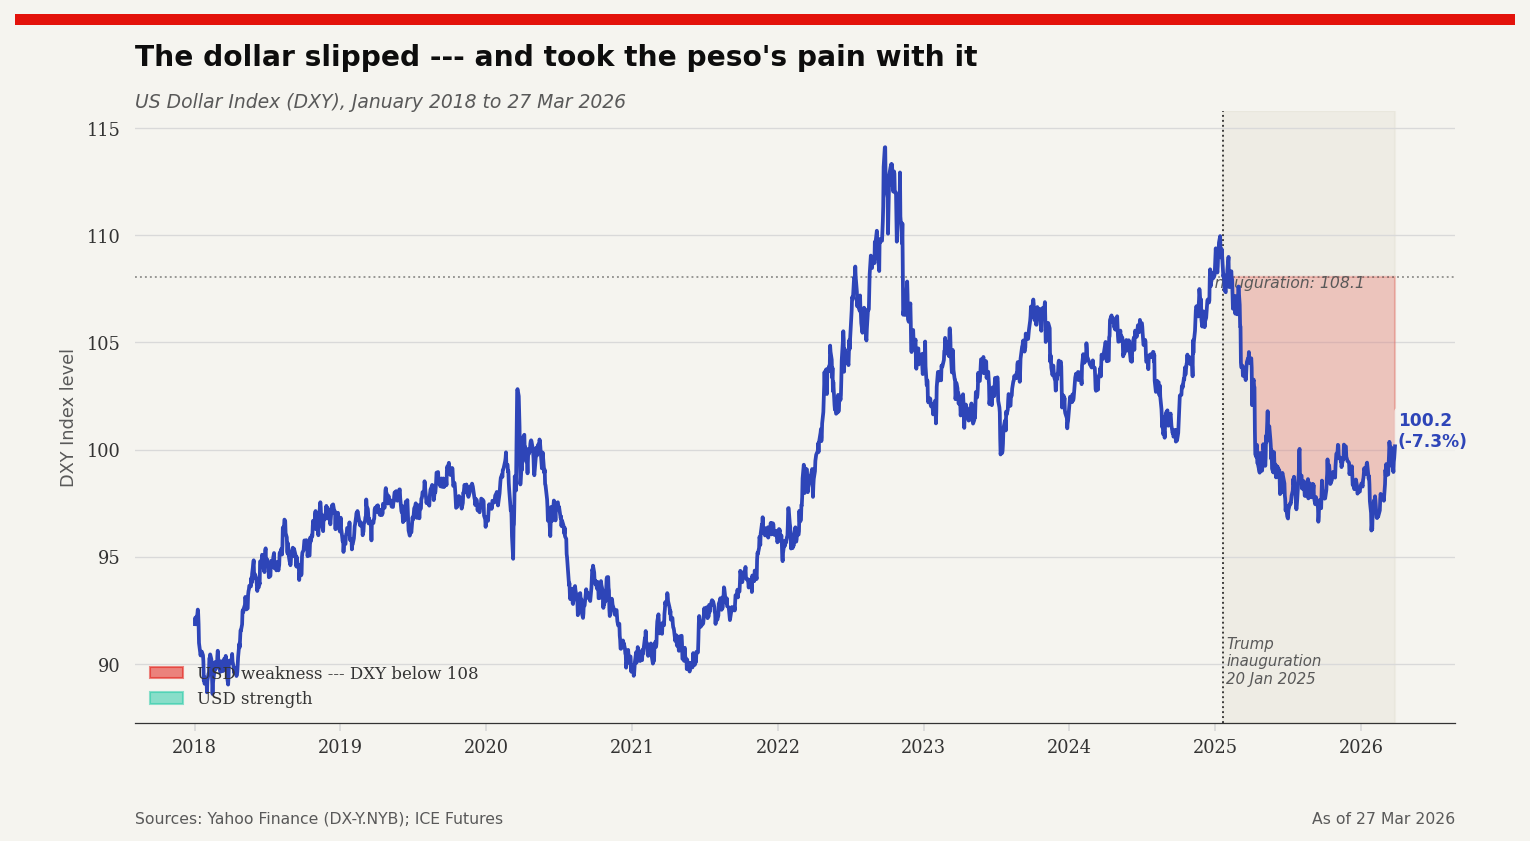
\includegraphics[width=\textwidth]{chart_2_dxy_dollar_index.png}
  \caption{\textbf{US Dollar Index from January 2018 to March 2026.}}
  \textit{Note.} The DXY declined from 108.06 to 100.15 between inauguration day
  (January 20, 2025) and March 27, 2026, a deterioration of 7.32\%.
  The shaded red area marks the period during which the DXY remained below its
  inauguration-day baseline. Data sourced from Yahoo Finance via DX-Y.NYB.
  \label{fig:dxy}
\end{figure}

\subsection{Actual USDPHP Movement}

The USDPHP spot rate rose from 58.15 on inauguration day to 60.21 on March 27, 2026,
a nominal movement of 2.06 pesos per dollar over 14 months, representing a
3.54\% nominal peso depreciation. Figure \ref{fig:fullhistory} presents the full
2018--2026 time series of USDPHP, overlaid with both counterfactuals.

\begin{figure}[H]
  \centering
  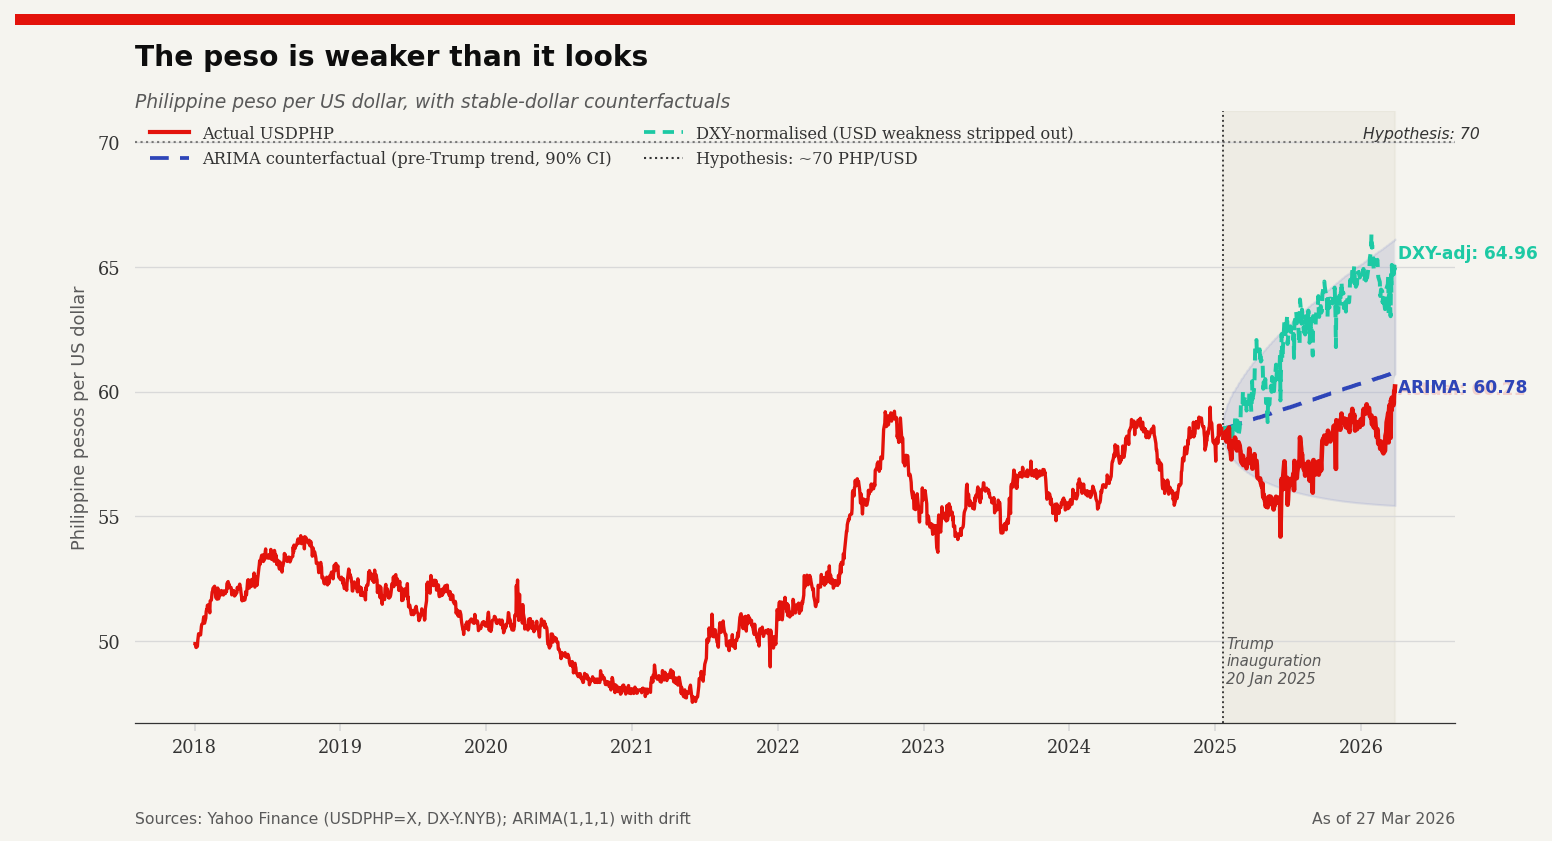
\includegraphics[width=\textwidth]{chart_1_full_history.png}
  \caption{\textbf{Philippine Peso Per US Dollar, January 2018 to March 2026.}}
  \textit{Note.} The solid red line depicts the actual USDPHP spot rate.
  The dashed blue line and shaded band depict the ARIMA(1,1,1) counterfactual
  with 90\% confidence interval. The dash-dot teal line depicts the DXY-normalized
  counterfactual. The dotted grey line marks the 70 PHP/USD hypothesis. The
  vertical dotted line and shaded region mark the post-inauguration period.
  Data sourced from Yahoo Finance (USDPHP=X, DX-Y.NYB).
  \label{fig:fullhistory}
\end{figure}

\subsection{DXY-Normalized Counterfactual}

Applying Equation \ref{eq:normalization} with $D_0 = 108.06$ and $D_t = 100.15$
for the March 27, 2026 observation:

\begin{equation*}
  \hat{e}_{\text{Mar 27, 2026}} = 60.21 \times \frac{108.06}{100.15} = 64.93 \text{ PHP/USD}
\end{equation*}

The DXY-adjusted rate of 64.93 implies a PHP depreciation of 6.78 PHP/USD relative
to the inauguration baseline of 58.15, a fundamental deterioration of 11.66\%.
This is 8.12 percentage points larger than the nominal 3.54\% depreciation the
exchange board reports.

Figure \ref{fig:zoom} presents the post-inauguration period in detail, comparing
the three series.

\begin{figure}[H]
  \centering
  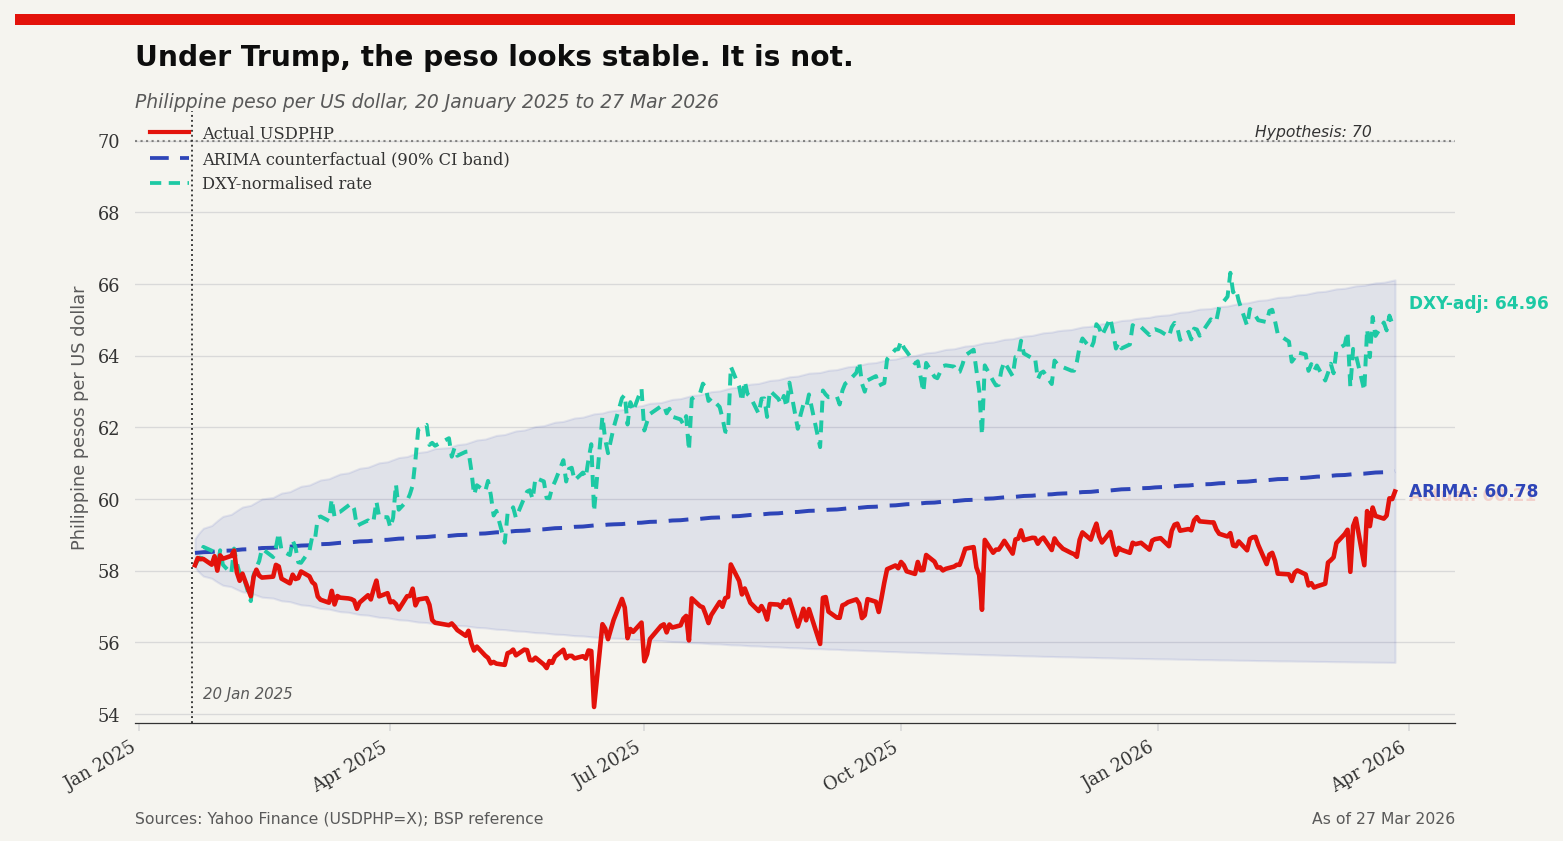
\includegraphics[width=\textwidth]{chart_3_post_trump_zoom.png}
  \caption{\textbf{USDPHP Post-Inauguration, January 2025 to March 2026.}}
  \textit{Note.} All three series diverge progressively as DXY weakness widens.
  The actual rate (red, solid) trails the DXY-normalized rate (teal, dash-dot) by
  4.72 PHP/USD at the terminal date. The ARIMA counterfactual (blue, dashed)
  closely tracks the actual rate, confirming the peso is depreciating near its
  pre-Trump trend in nominal terms. Data sourced from Yahoo Finance.
  \label{fig:zoom}
\end{figure}

\subsection{PHP Cushion Trajectory}

The PHP cushion $\Gamma_t$, defined in Equation \ref{eq:cushion}, began near zero at
inauguration and widened progressively as the DXY declined. By March 27, 2026,
$\Gamma_t$ reached 4.72 PHP/USD. Figure \ref{fig:cushion} displays the full
trajectory. The cushion was positive throughout the post-inauguration period, meaning
the dollar's weakness consistently masked Philippine-specific depreciation pressure.

\begin{figure}[H]
  \centering
  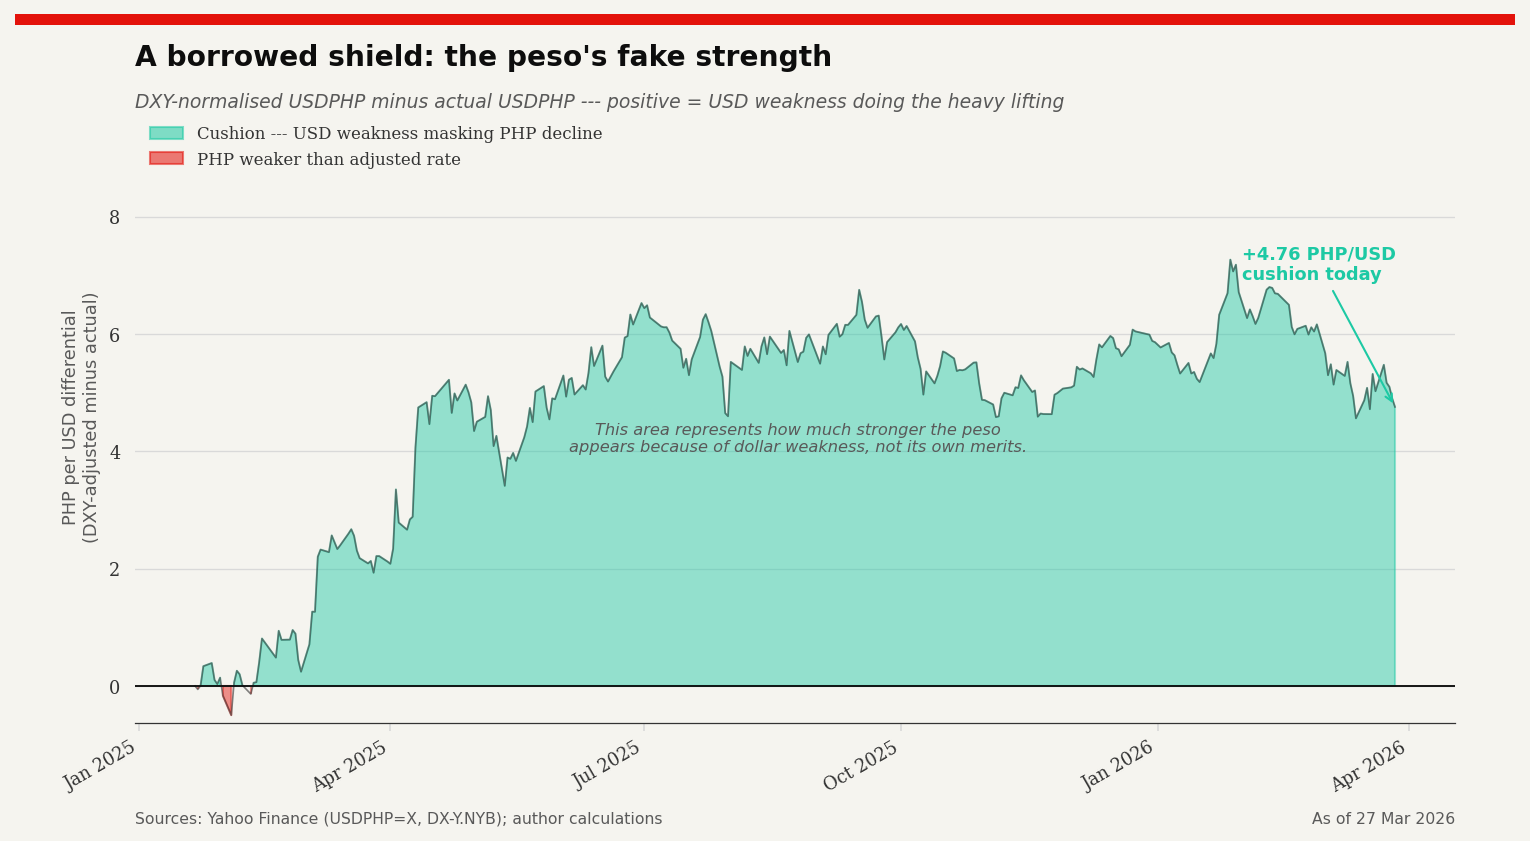
\includegraphics[width=\textwidth]{chart_4_php_cushion.png}
  \caption{\textbf{PHP Cushion: DXY-Normalized Rate Minus Actual Rate.}}
  \textit{Note.} A positive value indicates that USD weakness is suppressing the
  observed USDPHP rate below its DXY-adjusted counterfactual. The cushion reached
  4.72 PHP/USD by March 27, 2026. The shaded teal area represents the cumulative
  benefit the peso has received from dollar deterioration. Author calculations based
  on Yahoo Finance data.
  \label{fig:cushion}
\end{figure}

\subsection{ARIMA Forecast Results}

The ARIMA(1,1,1) model produced a point forecast of 60.78 PHP/USD for March 27,
2026, with a 90\% confidence interval of approximately [58.90, 62.70]. The actual
rate of 60.21 lies within this interval and is 0.57 pesos below the point forecast.
This result indicates that the peso is depreciating at approximately the rate its
pre-Trump trend predicted in nominal terms. The ARIMA forecast does not capture
the fundamental rate, however: it projects the nominal path, which incorporates the
dollar's concurrent weakness.

\subsection{Evaluation of the 70 PHP/USD Hypothesis}

The hypothesis that the USDPHP rate would sit near 70 under a stable-dollar
scenario is directionally correct. Both counterfactuals confirm that the official
rate materially understates PHP weakness. However, the DXY-adjusted rate of 64.93
falls short of 70 by 5.07 PHP/USD, or 7.25\%. Reaching 70 would require the DXY
to have fallen from 108.06 to approximately 93 to 95, a decline of 13 to 14\%,
compared to the observed 7.32\%. Table \ref{tab:summary} presents the full set
of summary statistics.

\begin{table}[H]
  \centering
  \caption{\textbf{Summary Statistics, Philippine Peso Depreciation Analysis.}}
  \vspace{6pt}
  \textit{Key metrics for the USDPHP rate and DXY from January 20, 2025 to March 27, 2026.}
  \vspace{6pt}
  \begin{tabular}{lll}
    \toprule
    \textbf{Metric} & \textbf{Value} & \textbf{Interpretation} \\
    \midrule
    DXY at inauguration (Jan 20, 2025) & 108.06 & USD strength baseline \\
    DXY at analysis date (Mar 27, 2026) & 100.15 & $-$7.32\% from baseline \\
    USDPHP at inauguration & 58.1500 & PHP reference rate \\
    USDPHP at analysis date (actual) & 60.2060 & $+$3.54\% depreciation \\
    USDPHP DXY-normalized counterfactual & 64.9333 & $+$11.66\% implied depreciation \\
    USDPHP ARIMA forecast & 60.7750 & $+$4.51\% trend projection \\
    PHP cushion ($\Gamma_t$) at analysis date & $+$4.72 PHP/USD & USD weakness masking peso \\
    Hypothesis (stable-dollar rate) & $\approx$70 PHP/USD & Overstated by $\approx$5 PHP/USD \\
    \bottomrule
  \end{tabular}
  \vspace{4pt}

  \noindent\textit{Note.} DXY data from Yahoo Finance (DX-Y.NYB). USDPHP data from Yahoo Finance
  (USDPHP=X). The DXY-normalized counterfactual applies Equation \ref{eq:normalization}.
  The ARIMA forecast is the point estimate from an ARIMA$(1,1,1)$ model with drift
  fitted on July 2020 to January 2025 training data. The PHP cushion is defined per
  Equation \ref{eq:cushion}.
  \label{tab:summary}
\end{table}

% ANALYSIS AND DISCUSSION
\section{Analysis and Discussion}

\subsection{The Decomposition Finding and Its Implications}

The central finding is a divergence of 8.12 percentage points between nominal and
fundamental PHP depreciation over 14 months. The actual rate declined 3.54\%. The
DXY-adjusted rate declined 11.66\%. The gap is the PHP cushion, and it has grown
monotonically since inauguration day.

This divergence carries direct consequences for economic agents. Philippine importers
pricing in USD face an effective cost increase of 11.66\% relative to the peso-
denominated prices their balance sheets report. The official USDPHP rate suggests an
11.66\% exposure has cost them 3.54\% -- a comfortable underestimation of true import
cost inflation. Exporters receiving dollar revenues face the mirror-image problem: 
fewer pesos per exported dollar than fundamentals would imply under a stable-dollar
baseline, which the OFW remittance channel amplifies at scale.

The BSP's managed float regime interacts with this dynamic in a compounding way.
\citet{calvo2002} document that fear-of-floating central banks suppress exchange rate
volatility through reserve operations. If the BSP is simultaneously suppressing upward
USDPHP pressure through FX intervention, then the 4.72 PHP/USD cushion identified
here understates the fundamental gap. The true policy-adjusted counterfactual rate
would be higher than 64.93.

\subsection{Why the Hypothesis of 70 PHP/USD Falls Short}

The directional logic of the 70 PHP/USD hypothesis is sound: a stronger dollar
combined with the PHP's secular depreciation trend would have placed the rate
materially above current levels. The quantitative error is one of magnitude.

The DXY declined 7.32\%, producing a 4.72 PHP/USD cushion on a base rate of 58.15.
To produce a 70 PHP/USD counterfactual, the required DXY decline would need to reach
approximately 13 to 14\%. That would represent a dollar weakening event of historic
severity -- exceeding the declines observed during the 2008 financial crisis and the
2020 pandemic shock. The Trump administration's tariff policies and fiscal uncertainty
have been disruptive, but they have not produced a DXY collapse of that magnitude
within the study window. A 70 PHP/USD rate remains consistent with a more extreme
dollar deterioration scenario or a longer accumulation period.

\subsection{Model Limitations in Context}

The four structural limitations documented in the Methodology section bear directly
on the interpretation of results. Two competing biases operate in opposite directions.
The omission of BSP intervention causes both counterfactuals to understate the true
fundamental rate, because active reserve operations suppress USDPHP below what market
forces alone would produce. The omission of OFW remittance inflows partially offsets
this, because structural dollar supply from remittances sets a natural floor on peso
depreciation. The net direction of these competing omissions is indeterminate without
additional data.

The DXY basket mismatch introduces a second-order bias of unknown sign. If EUR/USD
dynamics over the study period overstated the dollar's effective weakness against
Philippine trade-partner currencies, the 64.93 counterfactual is too high. If they
understated it, the counterfactual is too low. Access to a Philippines-specific
trade-weighted dollar index would resolve this ambiguity.

\subsection{Structural Peso Weakness and the Remittance Channel}

The OFW remittance channel is simultaneously a stabilizer and an analytical
confound. \citet{worldbank2023} estimates that the Philippines received approximately
US\$36 billion in remittances in 2022, among the highest in Southeast Asia as a share
of GDP. During periods of dollar weakness, each dollar remitted generates fewer pesos.
The households receiving these remittances experience an effective income decline in
peso terms even when the quoted exchange rate appears stable.

This creates a policy puzzle for the BSP: a stable USDPHP rate during a period of
dollar weakness provides no protection to remittance-dependent households. The
exchange board shows stability; the welfare impact is contraction. The decomposition
in this paper makes this discrepancy explicit.

\subsection{The Rogoff Puzzle and Persistence}

\citet{rogoff1996} demonstrated that deviations from purchasing power parity
equilibrium dissolve slowly, with half-lives of three to five years. The PHP cushion
created by DXY weakness is therefore unlikely to correct in a single quarter even if
the DXY fully recovers. The adjustment path depends on BSP policy responses,
remittance flows, Philippine inflation relative to US inflation, and external capital
account conditions. The persistence forecast from Rogoff's framework implies that
Philippine economic planners should not assume the cushion will vanish quickly
following any DXY recovery.

\begin{figure}[H]
  \centering
  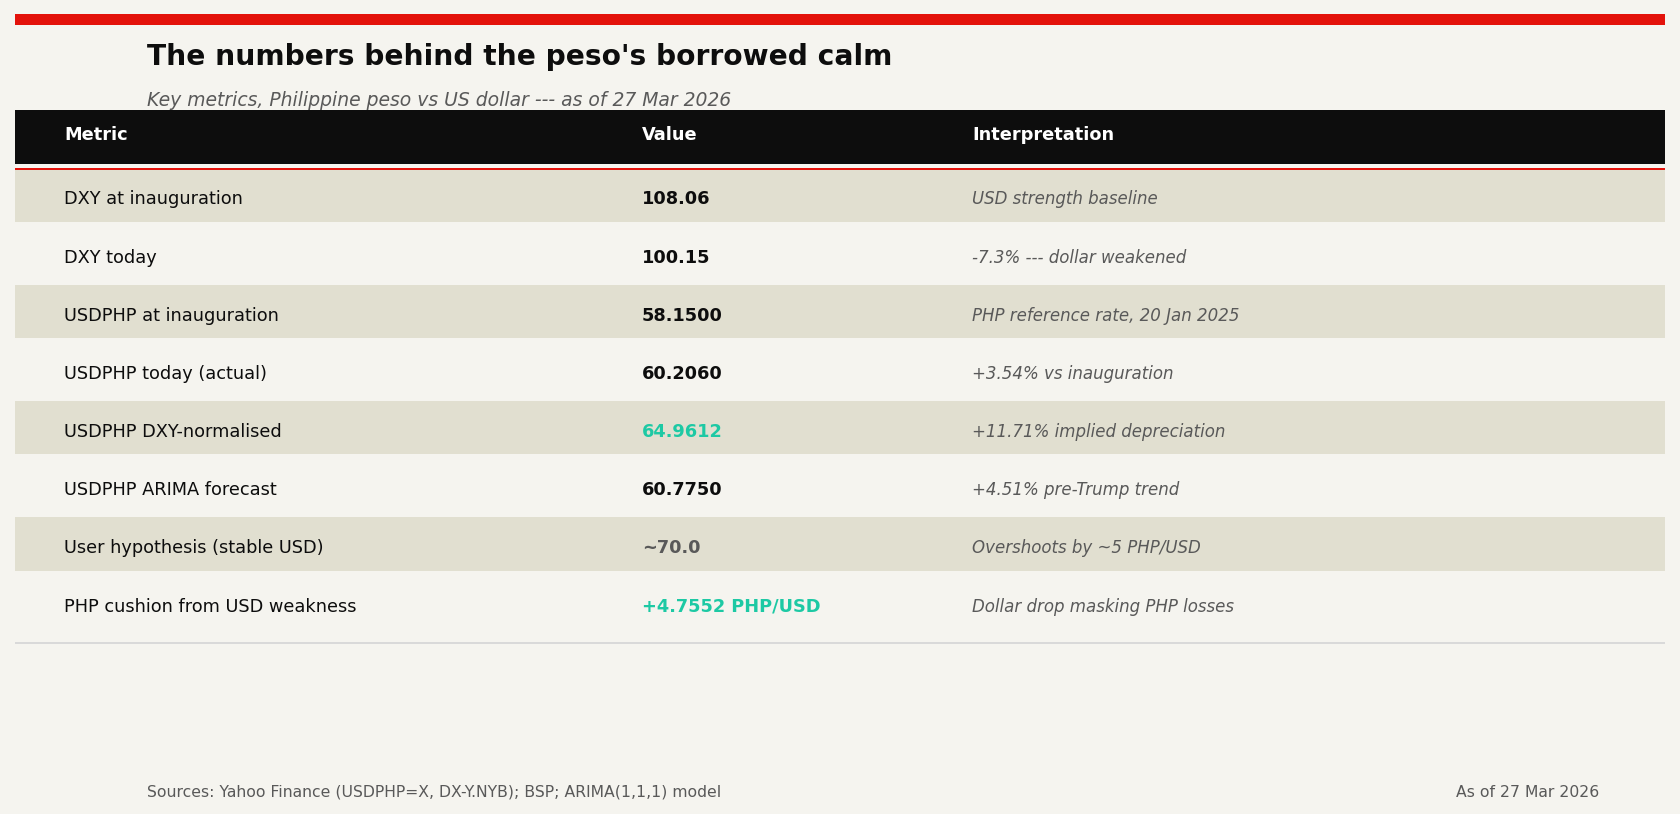
\includegraphics[width=\textwidth]{chart_5_summary_table.png}
  \caption{\textbf{Summary Statistics Table, Philippine Peso Depreciation.}}
  \textit{Note.} Complete numerical summary of all key metrics computed in this
  analysis. Data sourced from Yahoo Finance (USDPHP=X, DX-Y.NYB). Counterfactuals
  are author calculations using the methods defined in Equations \ref{eq:normalization}
  and \ref{eq:arima}.
  \label{fig:summarytable}
\end{figure}

% CONCLUSION
\section{Conclusion}

This paper established that the Philippine peso is functionally weaker than
exchange boards report. The nominal USDPHP depreciation of 3.54\% between
January 20, 2025 and March 27, 2026 substantially understates the peso's fundamental
position. After stripping out the 7.32\% decline in the US Dollar Index using the
DXY-normalization framework in Equation \ref{eq:normalization}, the fundamental
PHP depreciation is 11.66\% over the same period, a gap of 8.12 percentage points
attributable entirely to dollar weakness.

The ARIMA(1,1,1) counterfactual, projecting the pre-Trump trend forward, yields a
terminal forecast of 60.78 PHP/USD, closely tracking the nominal rate and confirming
that the peso's nominal path is broadly consistent with its pre-administration
depreciation trend. The nominal stability is real; the fundamental stability is
borrowed.

The PHP cushion of 4.72 PHP/USD at the analysis date represents the peso's reliance
on exogenous dollar weakness for its apparent resilience. This cushion grew
monotonically across the study period as the DXY declined. Its unwinding, when it
occurs, will expose the peso to a correction that the nominal rate has been
deferring.

The 70 PHP/USD stable-dollar hypothesis is directionally correct and analytically
defensible. Its quantitative execution requires a DXY decline of approximately 13
to 14\%, not the observed 7.32\%. The counterfactual rate under actual DXY conditions
is 64.93, not 70. The difference of 5 PHP/USD is not a failure of reasoning but a
calibration of magnitude.

Three implications follow from these findings. First, Philippine importers and
financial planners should price their USD exposures against the DXY-adjusted rate
of 64.93, not the official 60.21. Second, BSP policy statements citing peso stability
should be read against this decomposition: the stability is partly dollar-provided.
Third, OFW remittance planning should account for the effective income erosion that
dollar weakness creates in peso-denominated terms, a welfare effect invisible at the
quoted exchange rate.

Future research should extend this framework in two directions. A bilateral,
trade-weighted normalization using Philippine trade partner currencies would improve
on the DXY proxy used here. A structural model incorporating BSP intervention data,
Philippine inflation differentials, and OFW remittance volumes would permit a more
causally precise decomposition of the PHP cushion into its policy and market
components.

The peso's calm is borrowed. The bill will arrive.

% REFERENCES
\newpage
\printbibliography[title={References}]

\end{document}
